% ============================================================
%  CHAPITRE 3 : Approximations numériques pour la résolution des EDP
% ============================================================
\chapter{Approximations numériques pour la résolution des équations aux dérivées partielles}
\label{chap:approximations_numeriques}

\section{Introduction}
\label{sec:introduction_approx}

Les équations de Navier-Stokes sont largement utilisées pour modéliser le comportement des fluides. Toutefois, en tant qu'équations aux dérivées partielles (EDP) non linéaires, elles ne disposent pas de solution analytique générale. Pour cette raison, la résolution numérique constitue l'approche privilégiée afin d'obtenir des solutions approchées \cite{hirsch2007numerical}.

Parmi les techniques numériques les plus courantes, les méthodes des différences finies, des volumes finis et des éléments finis permettent de discrétiser le problème continu en un système algébrique traitable \cite{tannehill1997computational}.

\section{Méthode des différences finies}
\label{sec:differences_finies}

La méthode des différences finies consiste à approximer les dérivées des équations physiques à l'aide des séries de Taylor, en s'appuyant directement sur la définition mathématique de la dérivée \cite{smith1985numerical}.

\begin{figure}[H]
    \centering
    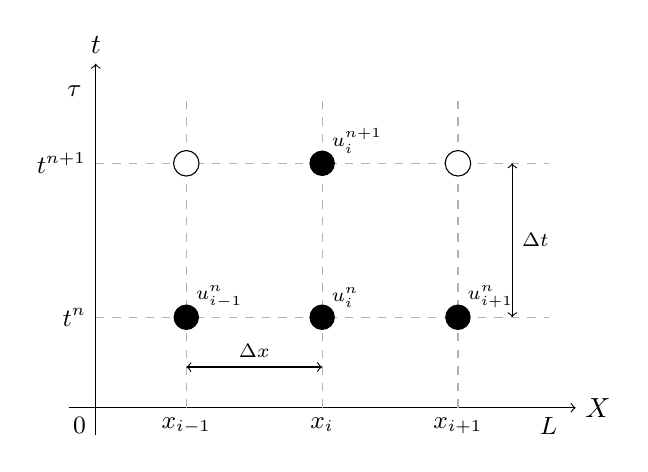
\begin{tikzpicture}[scale=1.15]
      % Axes
      \draw[->] (-0.3,0) -- (5.3,0) node[right] {$X$};
      \draw[->] (0,-0.3) -- (0,3.8) node[above] {$t$};
      \node[left, font=\small] at (-0.05,3.5) {$\tau$};
      % Positions x
      \def\xa{1.0} \def\xb{2.5} \def\xc{4.0}
      % Positions t
      \def\ta{1.0} \def\tb{2.7}
      % Lignes de grille verticales
      \draw[gray!60, dashed] (\xa,0) -- (\xa,3.4);
      \draw[gray!60, dashed] (\xb,0) -- (\xb,3.4);
      \draw[gray!60, dashed] (\xc,0) -- (\xc,3.4);
      % Lignes de grille horizontales
      \draw[gray!60, dashed] (0,\ta) -- (5.0,\ta);
      \draw[gray!60, dashed] (0,\tb) -- (5.0,\tb);
      % Étiquettes axe x
      \node[below, font=\small] at (\xa,0) {$x_{i-1}$};
      \node[below, font=\small] at (\xb,0) {$x_i$};
      \node[below, font=\small] at (\xc,0) {$x_{i+1}$};
      \node[below, font=\small] at (5.0,0) {$L$};
      \node[below left, font=\small] at (0,0) {$0$};
      % Étiquettes axe t
      \node[left, font=\small] at (0,\ta) {$t^n$};
      \node[left, font=\small] at (0,\tb) {$t^{n+1}$};
      % Points à t^n
      \fill (\xa,\ta) circle (4pt);
      \fill (\xb,\ta) circle (4pt);
      \fill (\xc,\ta) circle (4pt);
      % Points à t^{n+1}
      \fill (\xb,\tb) circle (4pt);
      \draw[fill=white] (\xa,\tb) circle (4pt);
      \draw[fill=white] (\xc,\tb) circle (4pt);
      % Étiquettes des n\oe uds
      \node[above right, font=\scriptsize] at (\xa,\ta) {$u_{i-1}^n$};
      \node[above right, font=\scriptsize] at (\xb,\ta) {$u_i^n$};
      \node[above right, font=\scriptsize] at (\xc,\ta) {$u_{i+1}^n$};
      \node[above right, font=\scriptsize] at (\xb,\tb) {$u_i^{n+1}$};
      % Annotation \Delta x
      \draw[<->] (\xa,0.45) -- (\xb,0.45) node[midway, above, font=\scriptsize] {$\Delta x$};
      % Annotation \Delta t
      \draw[<->] (4.6,\ta) -- (4.6,\tb) node[midway, right, font=\scriptsize] {$\Delta t$};
    \end{tikzpicture}
    \caption{Maillage de la méthode des différences finies.}
    \label{fig:maillage_df}
\end{figure}

Pour une fonction $u(x)$, la dérivée première peut être approximée par différents schémas. En utilisant le développement en série de Taylor :

\begin{equation}
u(x + \Delta x) = u(x) + \Delta x \frac{\partial u}{\partial x} + \frac{\Delta x^2}{2} \frac{\partial^2 u}{\partial x^2} + \dots
\label{eq:taylor}
\end{equation}

On obtient :
\begin{itemize}
    \item \textbf{Schéma décentré avant} (ordre 1) : \( \left( \frac{\partial u}{\partial x} \right)_i \approx \frac{u_{i+1} - u_i}{\Delta x} \)
    \item \textbf{Schéma décentré arrière} (ordre 1) : \( \left( \frac{\partial u}{\partial x} \right)_i \approx \frac{u_i - u_{i-1}}{\Delta x} \)
    \item \textbf{Schéma centré} (ordre 2) : \( \left( \frac{\partial u}{\partial x} \right)_i \approx \frac{u_{i+1} - u_{i-1}}{2\Delta x} \)
\end{itemize}

La dérivée seconde est approximée par le schéma centré d'ordre 2 \cite{strikwerda2004finite} :

\begin{equation}
\left( \frac{\partial^2 u}{\partial x^2} \right)_i \approx \frac{u_{i+1} - 2u_i + u_{i-1}}{\Delta x^2}
\label{eq:derivee_seconde}
\end{equation}

\section{Méthode des éléments finis}
\label{sec:elements_finis}

La méthode des éléments finis vise à minimiser l'erreur générée lors de l'approximation d'un problème continu par sa formulation discrète \cite{zienkiewicz2013finite}. Le domaine est subdivisé en petits éléments de géométrie simple interconnectés en des points appelés "nœuds". La solution est recherchée sous forme d'une combinaison linéaire de fonctions de base locales \cite{reddy2006introduction} :

\begin{equation}
\Phi_h(x) = \sum_{i=1}^{n} \Phi_i(x)\, N_i
\label{eq:elements_finis}
\end{equation}

\begin{itemize}
    \item[--] \(\Phi_h(x)\) : solution approchée discrète sur le domaine
    \item[--] \(\Phi_i(x)\) : valeur nodale de la solution au n\oe ud \(i\)
    \item[--] \(N_i\) : fonction de forme (base) associée au n\oe ud \(i\)
    \item[--] \(n\) : nombre total de n\oe uds de l'élément
\end{itemize}

Cette méthode est très mathématique et peut être appliquée à des géométries variées, mais elle rencontre des obstacles lorsqu'il s'agit de termes non linéaires, ce qui limite son application en CFD \cite{hughes2012finite}.

\begin{figure}[H]
    \centering
    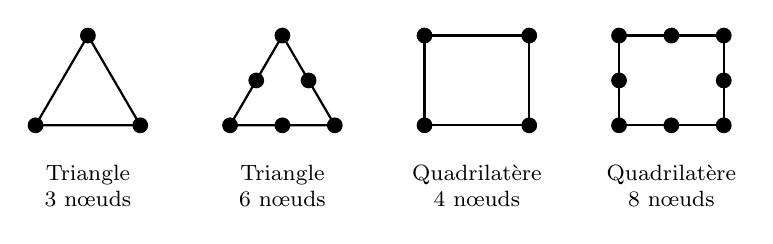
\begin{tikzpicture}[scale=0.95]
      % Triangle 3 n\oe uds
      \begin{scope}[xshift=0cm]
        \draw[thick] (0,0) -- (1.4,0) -- (0.7,1.2) -- cycle;
        \fill (0,0) circle (3pt); \fill (1.4,0) circle (3pt); \fill (0.7,1.2) circle (3pt);
        \node[below, font=\footnotesize, align=center] at (0.7,-0.4) {Triangle\\3 n\oe uds};
      \end{scope}
      % Triangle 6 n\oe uds
      \begin{scope}[xshift=2.6cm]
        \draw[thick] (0,0) -- (1.4,0) -- (0.7,1.2) -- cycle;
        \fill (0,0) circle (3pt); \fill (1.4,0) circle (3pt); \fill (0.7,1.2) circle (3pt);
        \fill (0.7,0) circle (3pt); \fill (1.05,0.6) circle (3pt); \fill (0.35,0.6) circle (3pt);
        \node[below, font=\footnotesize, align=center] at (0.7,-0.4) {Triangle\\6 n\oe uds};
      \end{scope}
      % Quadrilat\`ere 4 n\oe uds
      \begin{scope}[xshift=5.2cm]
        \draw[thick] (0,0) -- (1.4,0) -- (1.4,1.2) -- (0,1.2) -- cycle;
        \fill (0,0) circle (3pt); \fill (1.4,0) circle (3pt);
        \fill (1.4,1.2) circle (3pt); \fill (0,1.2) circle (3pt);
        \node[below, font=\footnotesize, align=center] at (0.7,-0.4) {Quadrilat\`ere\\4 n\oe uds};
      \end{scope}
      % Quadrilat\`ere 8 n\oe uds
      \begin{scope}[xshift=7.8cm]
        \draw[thick] (0,0) -- (1.4,0) -- (1.4,1.2) -- (0,1.2) -- cycle;
        \fill (0,0) circle (3pt); \fill (0.7,0) circle (3pt); \fill (1.4,0) circle (3pt);
        \fill (1.4,0.6) circle (3pt); \fill (1.4,1.2) circle (3pt);
        \fill (0.7,1.2) circle (3pt); \fill (0,1.2) circle (3pt); \fill (0,0.6) circle (3pt);
        \node[below, font=\footnotesize, align=center] at (0.7,-0.4) {Quadrilat\`ere\\8 n\oe uds};
      \end{scope}
    \end{tikzpicture}
    \caption{Les géométries de référence de quelques éléments 2D courants.}
    \label{fig:elements_2d}
\end{figure}

\begin{figure}[H]
    \centering
    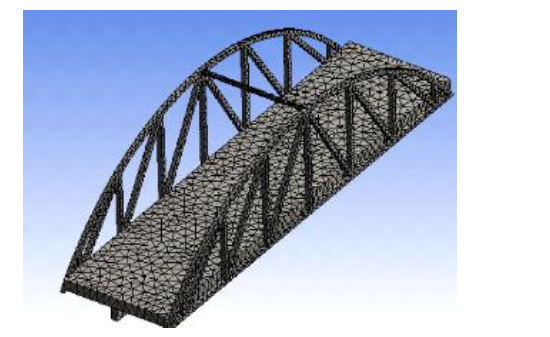
\includegraphics[width=0.6\textwidth]{figures/figure3_3.png}
    \caption{Maillage en éléments finis d'un pont de type Bow-string en vue d'une simulation.}
    \label{fig:maillage_pont}
\end{figure}

\section{Méthode des volumes finis}
\label{sec:volumes_finis}

La méthode des volumes finis repose sur l'intégration des équations en formulation intégrale sur des volumes élémentaires \cite{leveque2002finite}. Contrairement à la méthode des éléments finis, elle est particulièrement bien adaptée à la discrétisation spatiale des lois de conservation, ce qui en fait une méthode de choix en mécanique des fluides \cite{eymard2000finite}.

L'équation générale de transport pour une variable \( \phi \) s'écrit sous forme conservative \cite{moukalled2016finite} :

\begin{equation}
\frac{\partial}{\partial t}(\rho\phi) + \nabla\cdot(\rho\phi\vec{u}) = \nabla\cdot(\Gamma\nabla\phi) + S_\phi
\label{eq:transport_general}
\end{equation}

\begin{figure}[H]
    \centering
    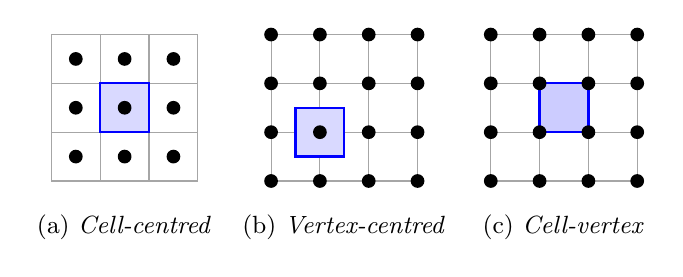
\begin{tikzpicture}[scale=0.62]
      % --- (a) Cell-centred ---
      \begin{scope}[xshift=0cm]
        \draw[gray!70, thin] (0,0) grid (3,3);
        \fill[blue!15] (1,1) rectangle (2,2);
        \draw[blue, thick] (1,1) rectangle (2,2);
        \foreach \x in {0.5,1.5,2.5} {
          \foreach \y in {0.5,1.5,2.5} {
            \fill (\x,\y) circle (4pt);
          }}
        \node[below, font=\small] at (1.5,-0.5) {(a) \textit{Cell-centred}};
      \end{scope}
      % --- (b) Vertex-centred ---
      \begin{scope}[xshift=4.5cm]
        \draw[gray!70, thin] (0,0) grid (3,3);
        \fill[blue!15] (0.5,0.5) rectangle (1.5,1.5);
        \draw[blue, thick] (0.5,0.5) rectangle (1.5,1.5);
        \foreach \x in {0,1,2,3} {
          \foreach \y in {0,1,2,3} {
            \fill (\x,\y) circle (4pt);
          }}
        \node[below, font=\small] at (1.5,-0.5) {(b) \textit{Vertex-centred}};
      \end{scope}
      % --- (c) Cell-vertex ---
      \begin{scope}[xshift=9.0cm]
        \draw[gray!70, thin] (0,0) grid (3,3);
        % Un seul carré encadré par 4 noeuds voisins
        \fill[blue!20] (1,1) rectangle (2,2);
        \draw[blue, thick] (1,1) rectangle (2,2);
        % Points aux sommets (vertices)
        \foreach \x in {0,1,2,3} {
          \foreach \y in {0,1,2,3} {
            \fill (\x,\y) circle (4pt);
          }}
        \node[below, font=\small] at (1.5,-0.5) {(c) \textit{Cell-vertex}};
      \end{scope}
    \end{tikzpicture}
    \caption{Comparaison des approches (a) \og Cell-centred\fg{}, (b) \og Vertex-centred\fg{}, (c) \og Cell-vertex\fg{}.}
    \label{fig:approches_vf}
\end{figure}

\begin{figure}[H]
    \centering
    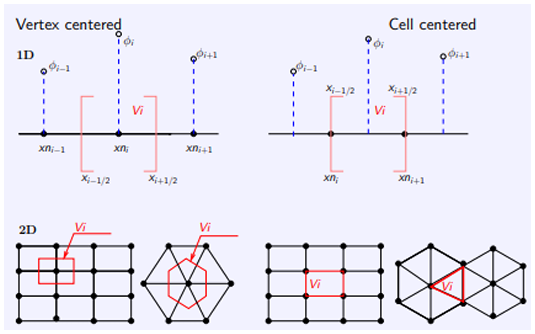
\includegraphics[width=0.6\textwidth]{figures/figure3_5.png}
    \caption{Exemples des volumes de contrôle en 1D et 2D.}
    \label{fig:volumes_controle_1d_2d}
\end{figure}

\begin{figure}[H]
    \centering
    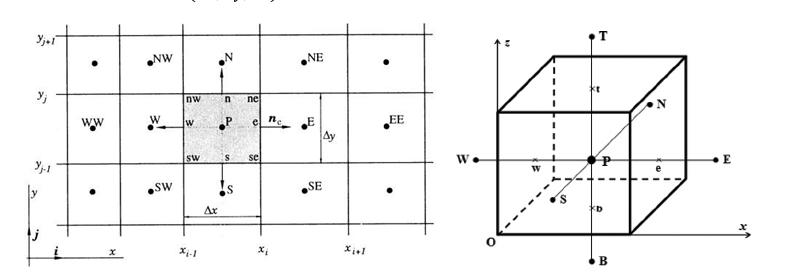
\includegraphics[width=0.6\textwidth]{figures/figure3_6.png}
    \caption{Exemple d'un volume de contrôle en 3D.}
    \label{fig:volume_controle_3d}
\end{figure}

\subsection{Discrétisation des termes de l'équation de transport}
\label{subsec:discretisation_termes}

\textbf{Discrétisation temporelle} : Le schéma d'Euler implicite, inconditionnellement stable mais précis au premier ordre, approxime la dérivée temporelle par \cite{butcher2016numerical} :

\begin{equation}
\int_V \frac{\partial (\rho\phi)}{\partial t} dV \approx \frac{(\rho\phi)_P^{n+1} - (\rho\phi)_P^n}{\Delta t} V_P
\label{eq:euler_implicite}
\end{equation}

\textbf{Terme de convection} : Il représente le transport de \( \phi \) par l'écoulement \cite{wesseling2001principles} :

\begin{equation}
\int_A \vec{n}\cdot(\rho\phi\vec{u})dA \approx \sum_f F_f \phi_f
\label{eq:convection}
\end{equation}

\textbf{Terme de diffusion} : Il représente le transport par gradient \cite{ferziger2002computational} :

\begin{equation}
\int_A \vec{n}\cdot(\Gamma\nabla\phi)dA \approx \sum_f \Gamma_f (\vec{n}\cdot\nabla\phi)_f A_f
\label{eq:diffusion}
\end{equation}

\subsection{Les schémas de discrétisation}
\label{subsec:schemas_discretisation}

\textbf{Schéma Upwind du premier ordre} : Stable et conservatif, ce schéma prend la valeur amont sans considération aval \cite{patankar1980numerical} :

\begin{equation}
\phi_e = \phi_P \text{ si } F_e > 0, \quad \phi_e = \phi_E \text{ si } F_e < 0
\label{eq:upwind}
\end{equation}

\begin{figure}[H]
    \centering
    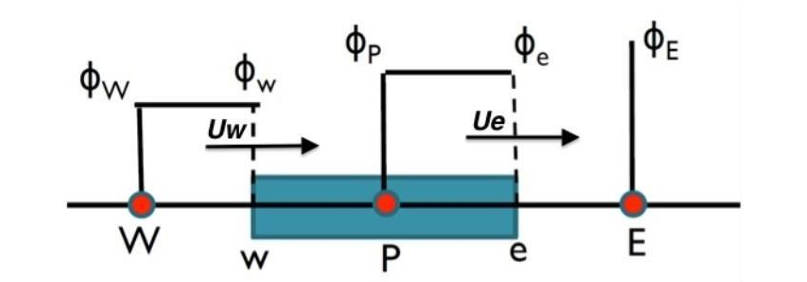
\includegraphics[width=0.6\textwidth]{figures/figure3_7.png}
    \caption{Schéma Upwind du 1er ordre.}
    \label{fig:upwind}
\end{figure}

\textbf{Schéma linéaire centré} : Plus précis (ordre 2), il utilise l'interpolation linéaire \cite{leonard1979stable} :

\begin{equation}
\phi_f = \frac{\phi_P + \phi_E}{2}
\label{eq:centre}
\end{equation}

\begin{figure}[H]
    \centering
    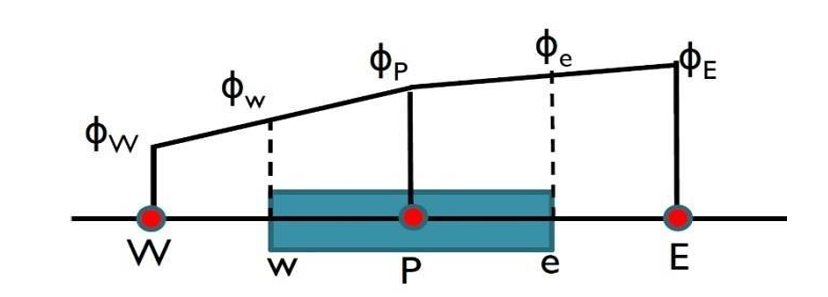
\includegraphics[width=0.6\textwidth]{figures/figure3_8.png}
    \caption{Schéma linéaire centré.}
    \label{fig:centre}
\end{figure}

\textbf{Schéma QUICK} : Proposé par Leonard \cite{leonard1991ultimate}, ce schéma d'ordre 3 utilise une interpolation quadratique pondérée :

\begin{equation}
\phi_e = \frac{6}{8}\phi_P + \frac{3}{8}\phi_E - \frac{1}{8}\phi_W \quad \text{pour } F_e > 0
\label{eq:quick}
\end{equation}

\begin{figure}[H]
    \centering
    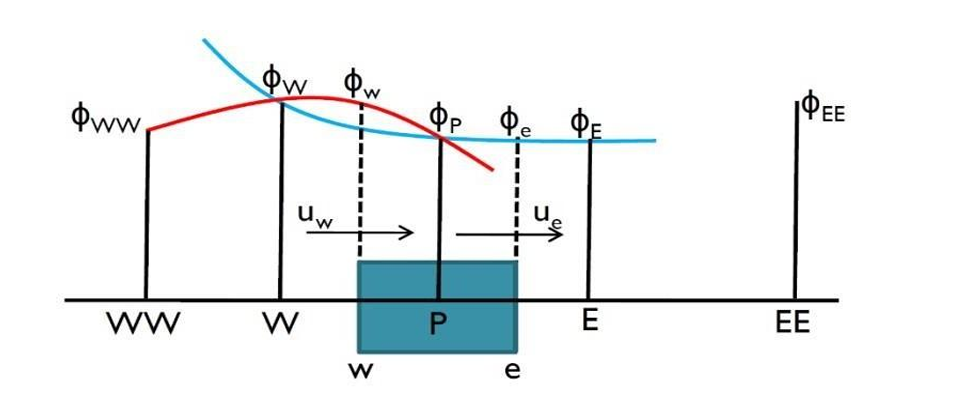
\includegraphics[width=0.6\textwidth]{figures/figure3_9.png}
    \caption{Schéma QUICK.}
    \label{fig:quick}
\end{figure}

\section{Conclusion}
\label{sec:conclusion_chap3}

Ce chapitre a introduit les diverses méthodes d'approximation numérique pour résoudre les équations de Navier-Stokes utilisées dans la modélisation hydraulique. Nous avons examiné les méthodes des différences finies, des éléments finis et des volumes finis. Ces méthodes constituent la base des outils de simulation numérique en hydraulique, et il est essentiel de choisir la méthode appropriée en fonction des caractéristiques du problème à résoudre. Dans notre cas, nous utiliserons la méthode des volumes finis qui est la méthode adoptée par OpenFOAM.
